\documentclass[12pt,a4paper]{report}

% Packages
\usepackage[a4paper, left=1.5in, right=1in, top=1in, bottom=1in]{geometry}
\usepackage{setspace}
\usepackage{titlesec}
\usepackage{fancyhdr}
\usepackage{times}
\usepackage{caption}
\usepackage{graphicx}
\usepackage{longtable}
\usepackage{booktabs}
\usepackage{lipsum} % for dummy text

% Line spacing
\onehalfspacing

% Page number style
\pagestyle{fancy}
\fancyhf{}
\fancyfoot[C]{\thepage}

% Chapter and section font size adjustments
\titleformat{\chapter}[hang]{\bfseries\fontsize{16}{20}\selectfont}{\thechapter}{1em}{}
\titleformat{\section}[hang]{\bfseries\fontsize{14}{16}\selectfont}{\thesection}{1em}{}
\titleformat{\subsection}[hang]{\bfseries\fontsize{14}{16}\selectfont}{\thesubsection}{1em}{}

% Table caption size
\captionsetup[figure]{font=footnotesize}

% Begin document
\begin{document}

% ----- Title Page -----
\begin{titlepage}
    \centering
    \vspace*{2cm}
    {\Huge\bfseries User Stories, Cases, and Requirements \par}
    \vspace{2cm}
    {\Large Project: rhymeo \par}
    \vspace{0.5cm}
    {\Large Version: 0.1 \par}
    \vspace{0.5cm}
    {\Large Team \#4: Doomsday \par}
    \vspace{0.5cm}
    {\Large Joshua Lester\par}
    \vspace{0.5cm}
    {\large CSCD350: Software Development Principles \par}
    \vspace{0.5cm}
    {\Large Instructor: Dr. Sanmeet Kaur \par}
    \vspace{0.5cm}
    \vfill
    {\Large Date: \today \par}
\end{titlepage}

% ----- Content -----
\chapter{Assignment}

\section{User Stories}
\begin{enumerate}

    \item As an app user, I want to be able to input my lyrics as a text file, so I don't have to type them in manually.
    \item As an app user, I want to receive error messages when I've inputted the wrong format, so I can fix the error with ease.
    \item As an app user, I want to be able receive help from the app if I don't understand exactly how to use it.
    \item As an app user, I want to be able to tell the app what to do.
    \item As an app user, I want the app to separate the lyrics into words, syllables, and pronunciation so that I can understand the pronunciation structure.
    \item As an app user, I want the app to remember what words I've inputted before so it can deliver my rhyme scheme faster.
    \item As an app user, I want to be able to see my rhyme scheme visualized with colors to benefit my writing process.
    \item As an app user, I want to be able to go through an installation process that makes everything easy to use so I don't have to keep track of the internals of the app.
    \item As an app user, I want to be able to look up potential rhymes so I can be assisted in my writing process.
    \item As an app user, I want to be able to use the app through a visual representation, so I can use it easier.
    \item As an app user, I don't want to worry about formatting the lyrics perfectly (without punctuation), in order to make the process easier.
\end{enumerate}

\section{Use Case Diagram}
\begin{figure}[h]
    \centering
    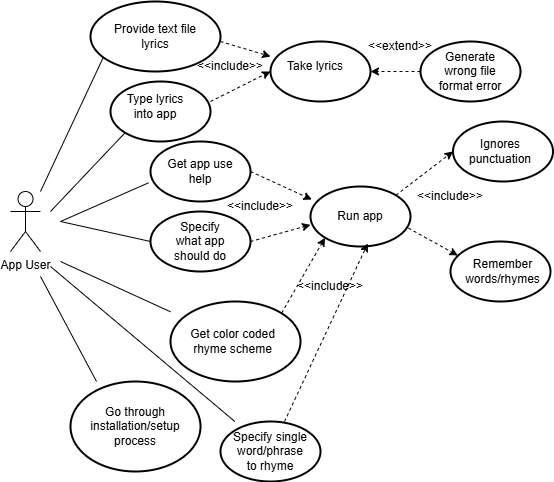
\includegraphics[width=0.75\textwidth]{use-case-diagram.png}
    \caption{Use Case Diagram}
\end{figure}
% ----- Table Example -----
\section{Requirements and Specifications}
\begin{enumerate}
    \item There will be a feature to intake lyrics through the command line.
    \item There will be a feature to intake lyrics through the command line as a file. This feature will use another software tool for reading files.
    \item There will also be a feature to intake lyrics as the user types them out. This feature will use another software tool for keeping track of the lyrics.
    \item There will be a feature let the user know about errors such as wrong file format.
    \item There will be a feature to ask the app for help.
    \item There will be a feature to find out what the user wants the app to do (as there might be multiple modes).
    \item There will be a feature to divide the lyrics into lines, words, syllables, and then into pronunciation for better analyzation. This feature will rely on a pronunciation dictionary.
    \item There will be a feature to store words from pronouncing dictionary and past words inputted and rhymes found into storage in the app.
    \item There will be a feature to color the lyrics in the console text. This feature will use a tool for coloring text.
    \item There will be a feature to run through an installation process, to keep the maintenance of the app clean and easy.
    \item There will be a feature to query the application on words that rhyme with a user-given word.
    \item There will be a feature to parse the lyrics and ignore values that aren't essential to the analyzation of the lyrical content (such as punctuation). The app will also put the nonessential characters back to maintain integrity of lyrics/input.
\end{enumerate}
% ----- Figure Example -----
\section{Glossary}
\begin{enumerate}
    \item Syllable: unit of pronunciation having one vowel sound.
    \item Rhyme scheme: a poem or song's rhythm in each line or word in relation to other lines or words.
    \item Pronouncing dictionary: dictionary used for lookups for pronunciation. Sometimes used by new language learners to help with correct pronunciation.
\end{enumerate}

\end{document}

